\documentclass[11pt]{article}
\usepackage[textwidth=18.0cm, textheight=23.0cm, top=2.0cm]{geometry}
\usepackage{pst-all}
\usepackage{amssymb}
\usepackage{tikz}
\usepackage{underscore}\begin{document}
\pagestyle{empty}


ClassName: \underline{\textbf{Class_10.2bp-8}}
\par
BinSize: \underline{\textbf{100 × 100}}
\par
ReduceSize: \underline{\textbf{100 × 100}}
\par
TypeNum: \underline{\textbf{20}}
\par
Num: \underline{\textbf{20}}
\par
OutS: \underline{\textbf{50000}}
\par
InS: \underline{\textbf{43948}}
\par
Rate: \underline{\textbf{0.879}}
\par
UB: \underline{\textbf{5}}
\par
LB0: \underline{\textbf{5}}
\par
LB: \underline{\textbf{5}}
\par
LBWithCut: \underline{\textbf{5}}
\par
NodeCut: \underline{\textbf{0}}
\par
ExtendedNodeCnt: \underline{\textbf{1}}
\par
GenNodeCnt: \underline{\textbf{1}}
\par
PrimalNode: \underline{\textbf{0}}
\par
ColumnCount: \underline{\textbf{5}}
\par
TotalCutCount: \underline{\textbf{0}}
\par
RootCutCount: \underline{\textbf{0}}
\par
LPSolverCnt: \underline{\textbf{1}}
\par
PricingSolverCnt: \underline{\textbf{0}}
\par
BranchAndBoundNum: \underline{\textbf{1}}
\par
isOpt: \underline{\textbf{true}}
\par
TimeOnPrimal: \underline{\textbf{0.000 s}}
\par
TimeOnPricing: \underline{\textbf{0.000 s}}
\par
TimeOnRmp: \underline{\textbf{0.062 s}}
\par
TotalTime: \underline{\textbf{0.109 s}}
\par
\newpage


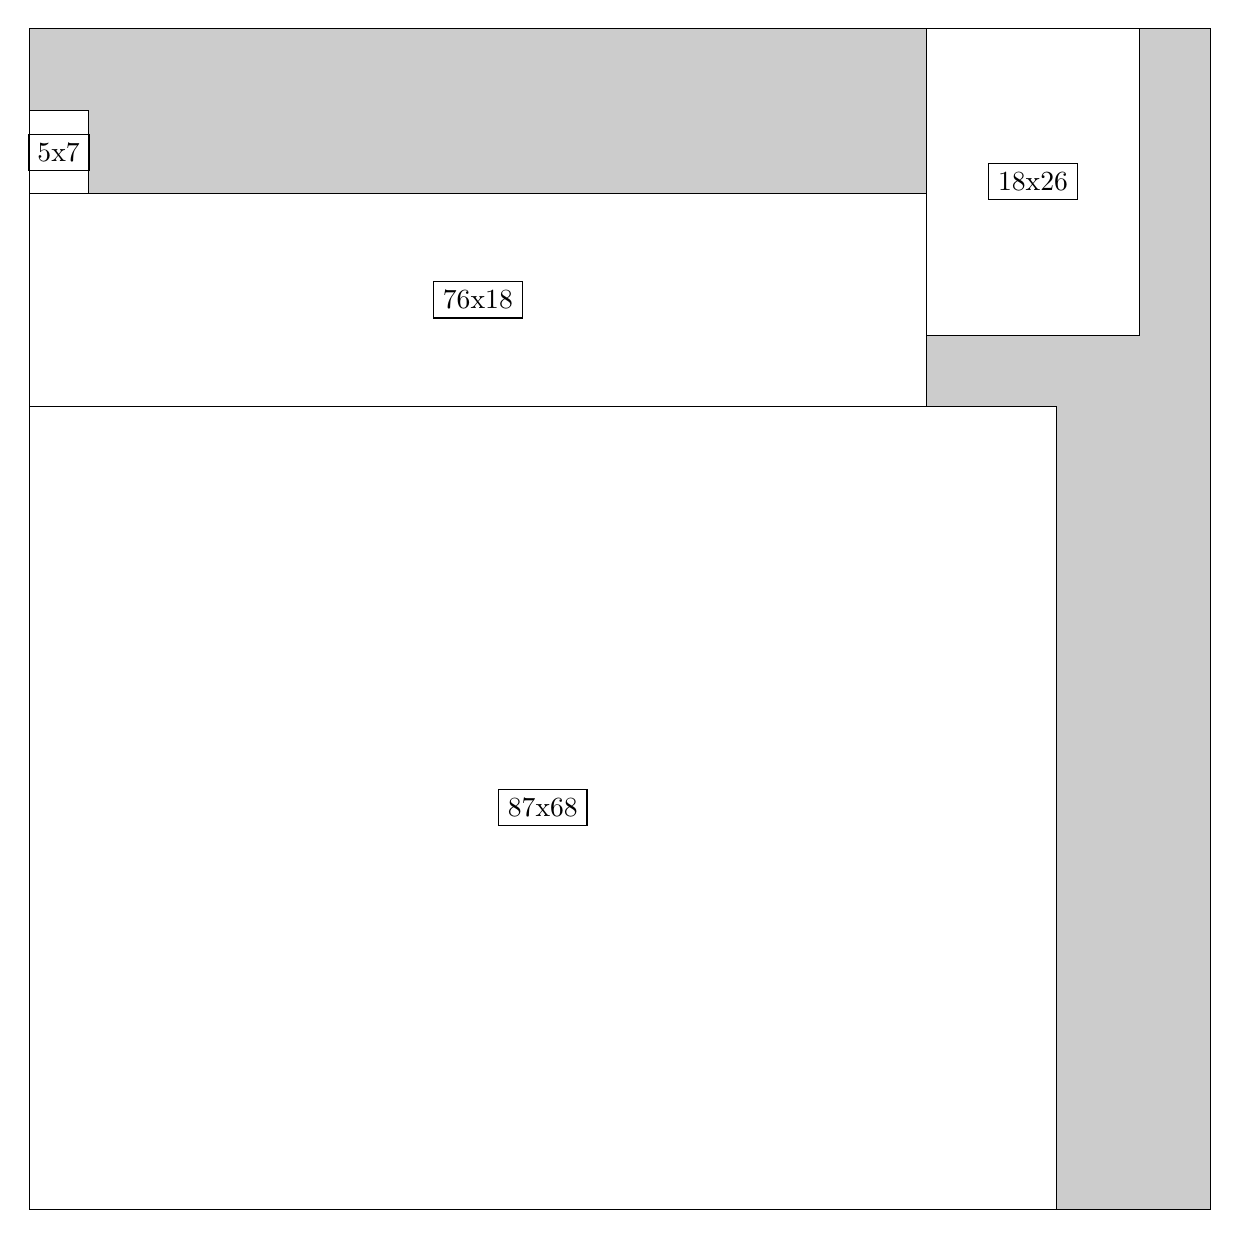
\begin{tikzpicture}[shorten >=1pt,scale=1.0,every node/.style={scale=1.0},->]
\tikzstyle{vertex}=[circle,fill=black!25,minimum size=14pt,inner sep=0pt]
\filldraw[fill=gray!40!white, draw=black] (0,0) rectangle (15.0,15.0);
\foreach \name/\x/\y/\w/\h in {87x68/0.0/0.0/13.049999999999999/10.2,76x18/0.0/10.2/11.4/2.6999999999999997,5x7/0.0/12.9/0.75/1.05,18x26/11.4/11.1/2.6999999999999997/3.9}
\filldraw[fill=white!40!white, draw=black] (\x,\y) rectangle node[draw] (\name) {\name} ++(\w,\h);
\end{tikzpicture}


w =87 , h =68 , x =0 , y =0 , v =5916
\par
w =76 , h =18 , x =0 , y =68 , v =1368
\par
w =5 , h =7 , x =0 , y =86 , v =35
\par
w =18 , h =26 , x =76 , y =74 , v =468
\par
\newpage


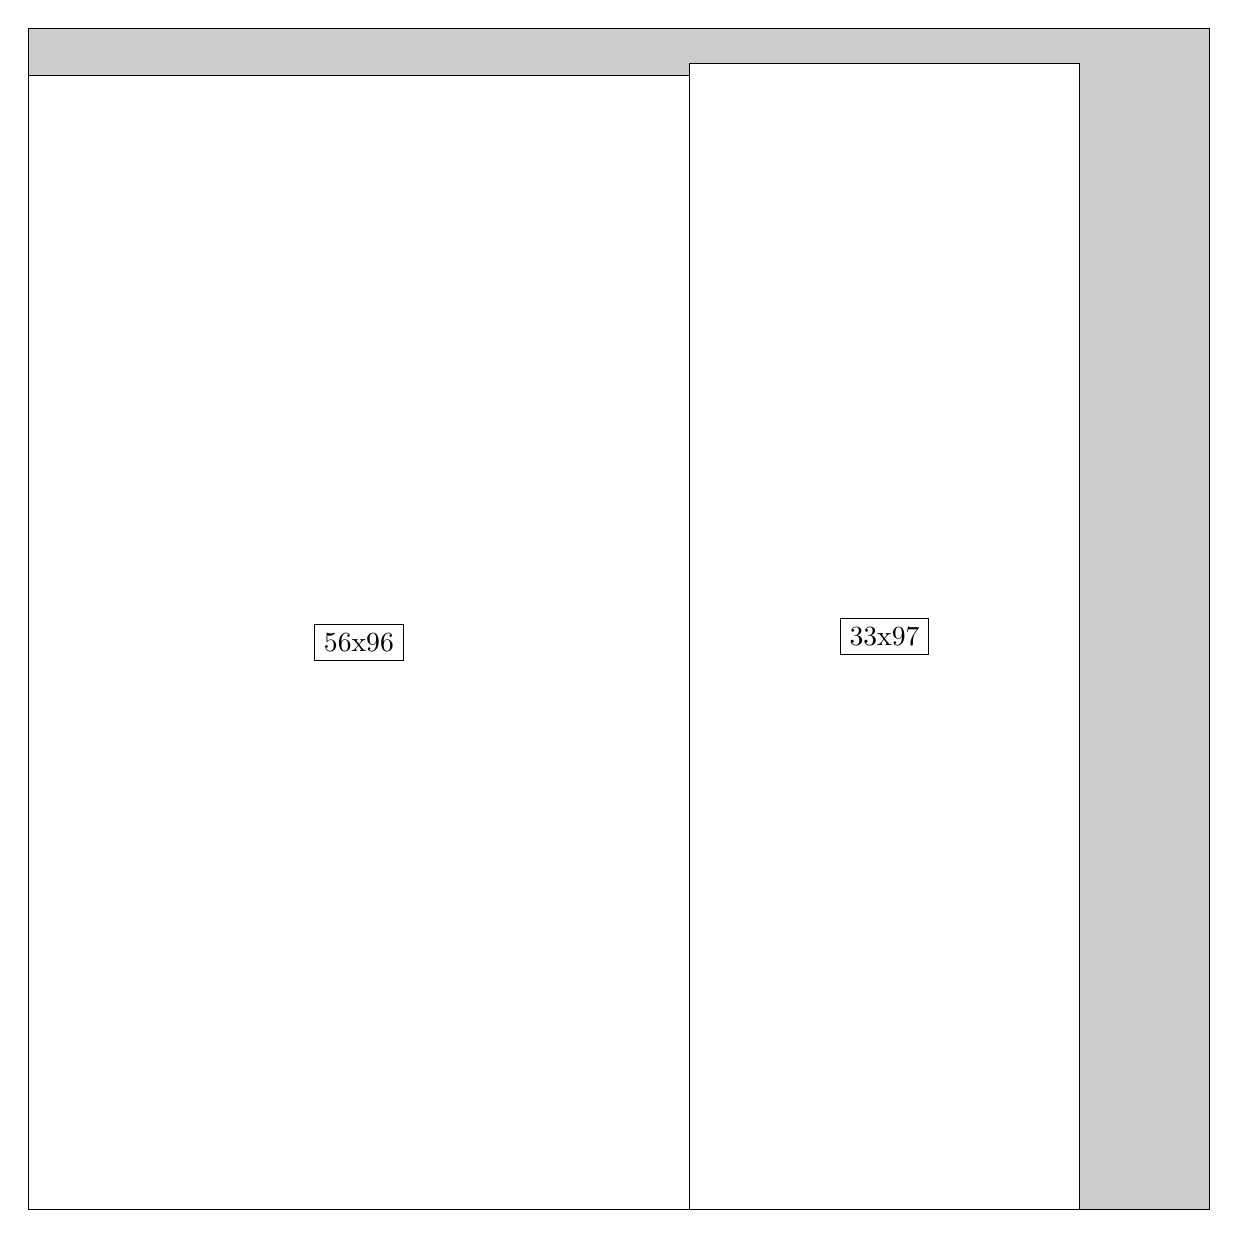
\begin{tikzpicture}[shorten >=1pt,scale=1.0,every node/.style={scale=1.0},->]
\tikzstyle{vertex}=[circle,fill=black!25,minimum size=14pt,inner sep=0pt]
\filldraw[fill=gray!40!white, draw=black] (0,0) rectangle (15.0,15.0);
\foreach \name/\x/\y/\w/\h in {33x97/8.4/0.0/4.95/14.549999999999999,56x96/0.0/0.0/8.4/14.399999999999999}
\filldraw[fill=white!40!white, draw=black] (\x,\y) rectangle node[draw] (\name) {\name} ++(\w,\h);
\end{tikzpicture}


w =33 , h =97 , x =56 , y =0 , v =3201
\par
w =56 , h =96 , x =0 , y =0 , v =5376
\par
\newpage


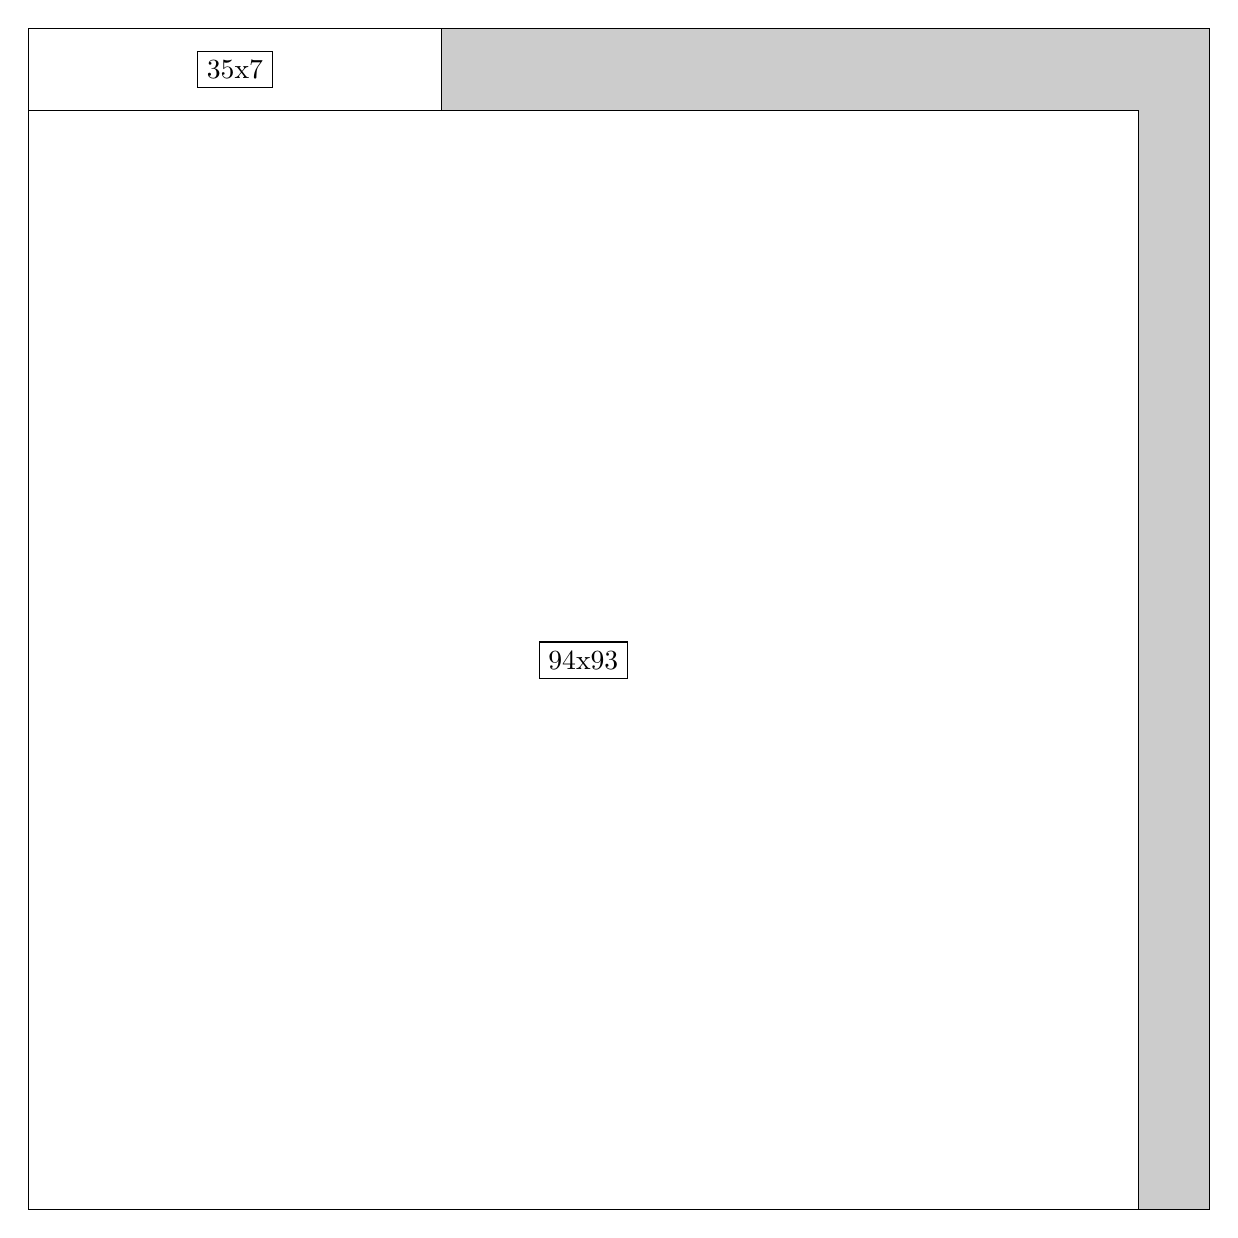
\begin{tikzpicture}[shorten >=1pt,scale=1.0,every node/.style={scale=1.0},->]
\tikzstyle{vertex}=[circle,fill=black!25,minimum size=14pt,inner sep=0pt]
\filldraw[fill=gray!40!white, draw=black] (0,0) rectangle (15.0,15.0);
\foreach \name/\x/\y/\w/\h in {35x7/0.0/13.95/5.25/1.05,94x93/0.0/0.0/14.1/13.95}
\filldraw[fill=white!40!white, draw=black] (\x,\y) rectangle node[draw] (\name) {\name} ++(\w,\h);
\end{tikzpicture}


w =35 , h =7 , x =0 , y =93 , v =245
\par
w =94 , h =93 , x =0 , y =0 , v =8742
\par
\newpage


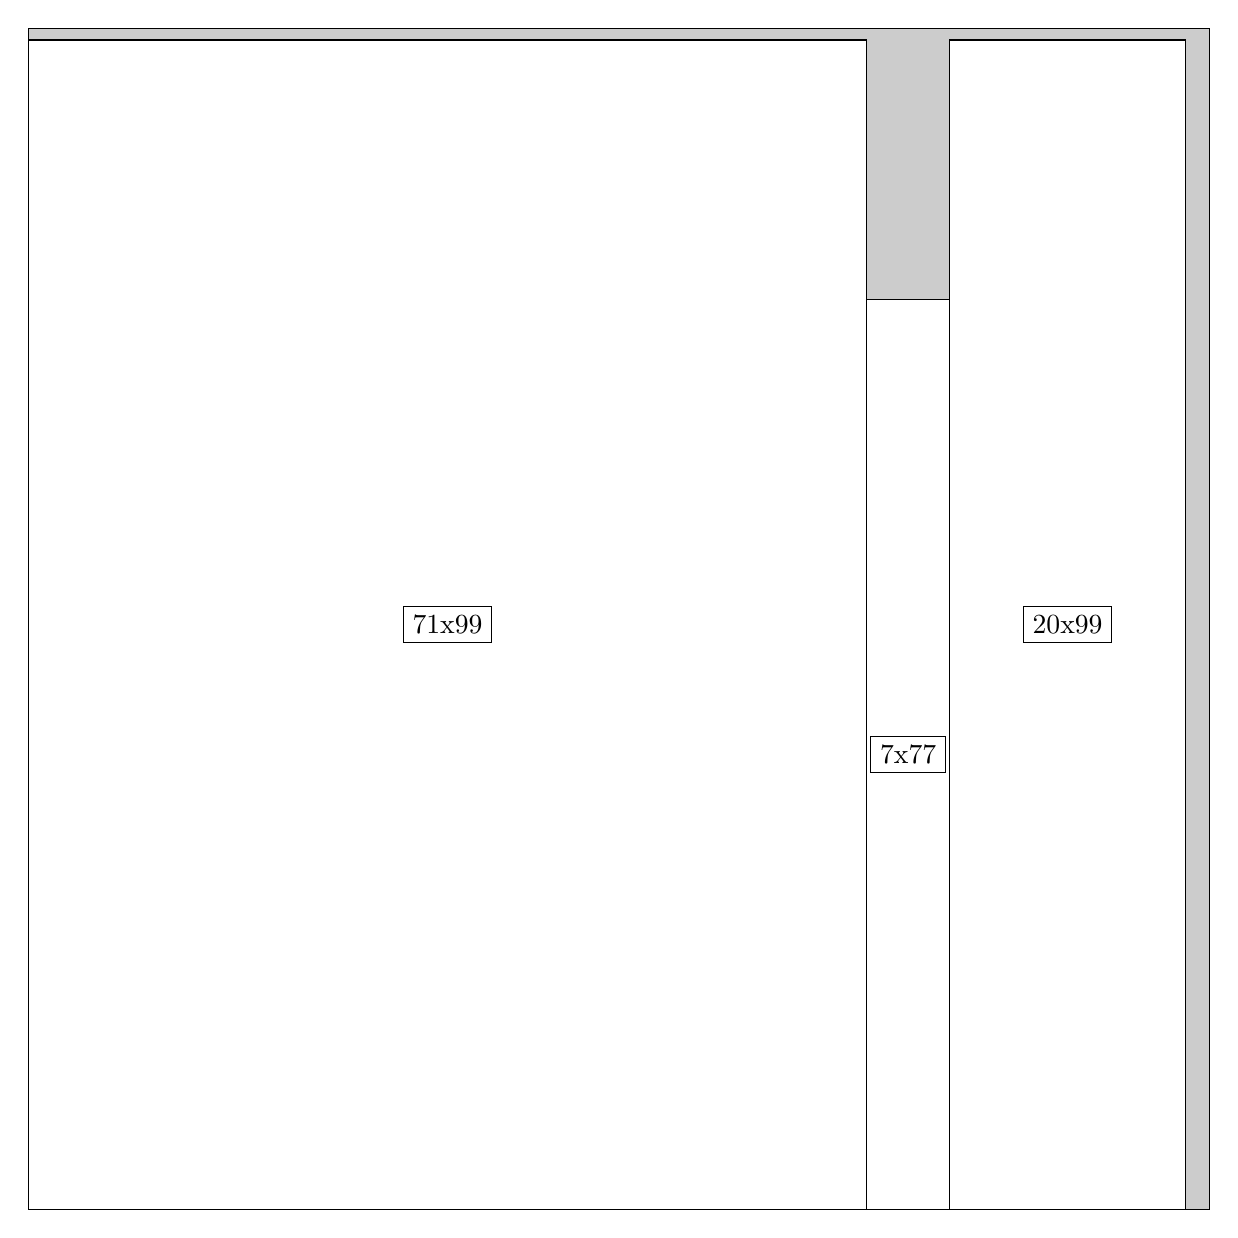
\begin{tikzpicture}[shorten >=1pt,scale=1.0,every node/.style={scale=1.0},->]
\tikzstyle{vertex}=[circle,fill=black!25,minimum size=14pt,inner sep=0pt]
\filldraw[fill=gray!40!white, draw=black] (0,0) rectangle (15.0,15.0);
\foreach \name/\x/\y/\w/\h in {7x77/10.65/0.0/1.05/11.549999999999999,20x99/11.7/0.0/3.0/14.85,71x99/0.0/0.0/10.65/14.85}
\filldraw[fill=white!40!white, draw=black] (\x,\y) rectangle node[draw] (\name) {\name} ++(\w,\h);
\end{tikzpicture}


w =7 , h =77 , x =71 , y =0 , v =539
\par
w =20 , h =99 , x =78 , y =0 , v =1980
\par
w =71 , h =99 , x =0 , y =0 , v =7029
\par
\newpage


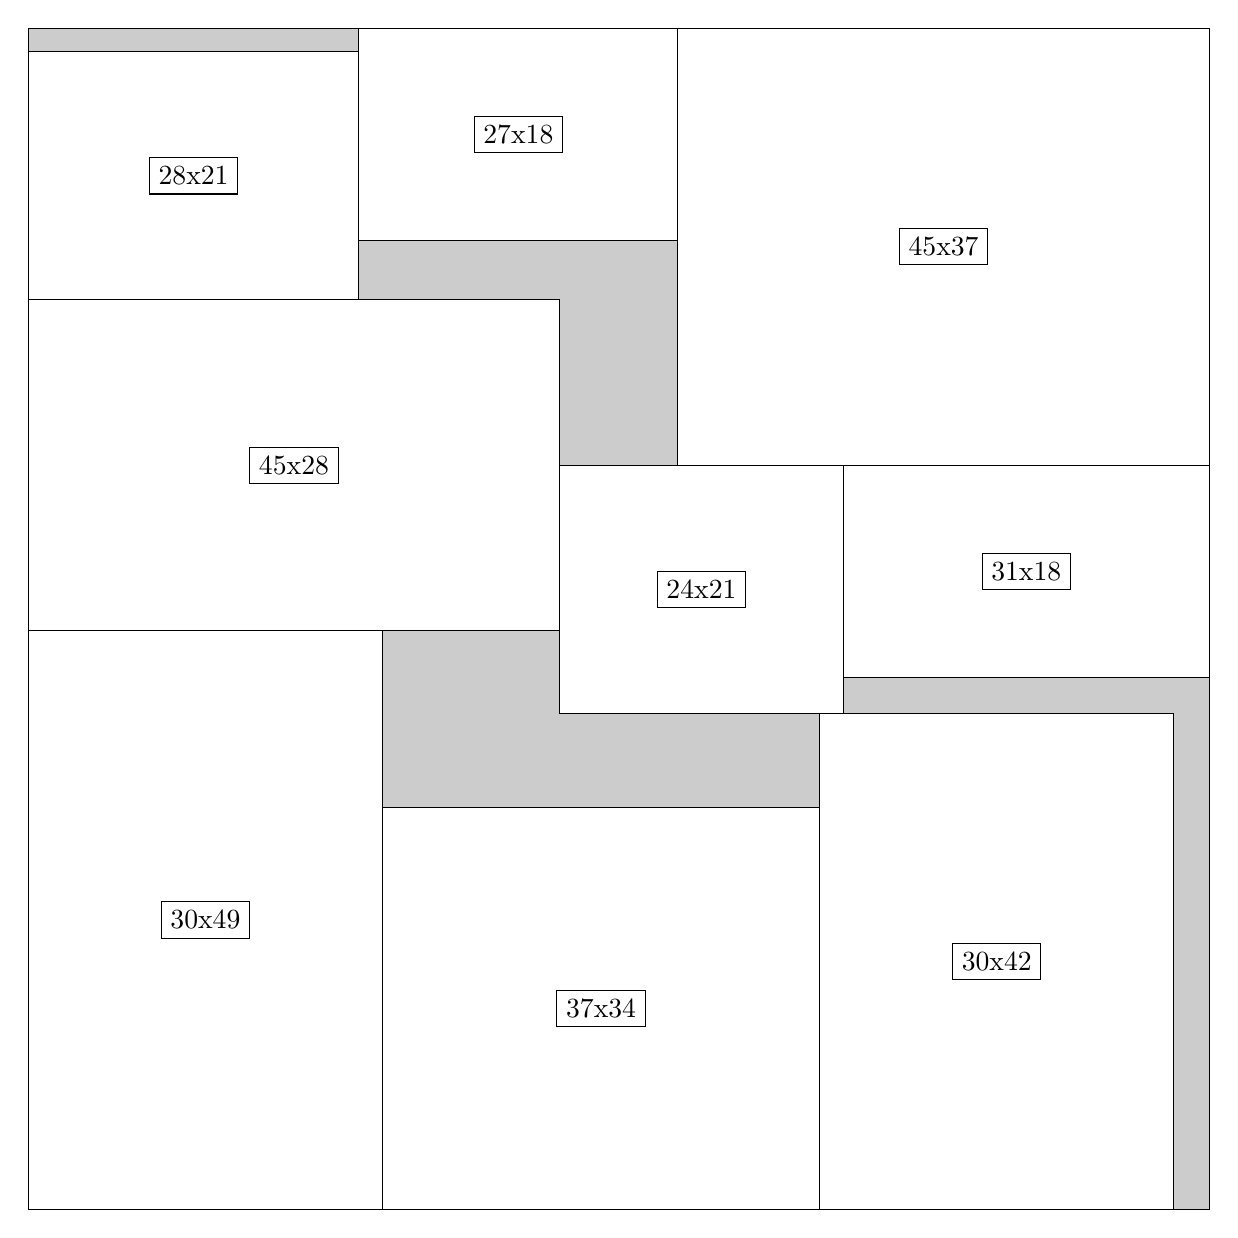
\begin{tikzpicture}[shorten >=1pt,scale=1.0,every node/.style={scale=1.0},->]
\tikzstyle{vertex}=[circle,fill=black!25,minimum size=14pt,inner sep=0pt]
\filldraw[fill=gray!40!white, draw=black] (0,0) rectangle (15.0,15.0);
\foreach \name/\x/\y/\w/\h in {30x49/0.0/0.0/4.5/7.35,45x28/0.0/7.35/6.75/4.2,37x34/4.5/0.0/5.55/5.1,30x42/10.049999999999999/0.0/4.5/6.3,28x21/0.0/11.549999999999999/4.2/3.15,27x18/4.2/12.299999999999999/4.05/2.6999999999999997,45x37/8.25/9.45/6.75/5.55,24x21/6.75/6.3/3.5999999999999996/3.15,31x18/10.35/6.75/4.6499999999999995/2.6999999999999997}
\filldraw[fill=white!40!white, draw=black] (\x,\y) rectangle node[draw] (\name) {\name} ++(\w,\h);
\end{tikzpicture}


w =30 , h =49 , x =0 , y =0 , v =1470
\par
w =45 , h =28 , x =0 , y =49 , v =1260
\par
w =37 , h =34 , x =30 , y =0 , v =1258
\par
w =30 , h =42 , x =67 , y =0 , v =1260
\par
w =28 , h =21 , x =0 , y =77 , v =588
\par
w =27 , h =18 , x =28 , y =82 , v =486
\par
w =45 , h =37 , x =55 , y =63 , v =1665
\par
w =24 , h =21 , x =45 , y =42 , v =504
\par
w =31 , h =18 , x =69 , y =45 , v =558
\par
\newpage


\end{document}